\documentclass[11pt, compress,xcolor=dvipsnames]{beamer}
\usepackage{booktabs}
\usepackage{color}
\usepackage{latexsym}
\usepackage{amsfonts}
\usepackage{amsmath}
\usepackage{multirow}
\usepackage[english]{babel}
\usepackage[utf8]{inputenc}
\usepackage{fancyhdr}
\usepackage{graphicx}
\usepackage{textcomp}
\usepackage{siunitx}
%\usepackage{bookmark}
%\usepackage{xcolor}
\usepackage{adjustbox}
% \usepackage{MnSymbol}

\usepackage{rotating}

%\usepackage{pstricks}
%\usepackage{pst-plot}

\usepackage{tikz}
\usepackage{tikzsymbols}
\usetikzlibrary{positioning,arrows,arrows.meta}
\usetikzlibrary{shapes.misc}
\tikzset{cross/.style={cross out, draw=black, minimum size=2*(#1-\pgflinewidth), inner sep=0pt, outer sep=0pt},
%default radius will be 1pt. 
cross/.default={1pt}} 
 

\definecolor{grigio}{gray}{0.25}
\newenvironment{sistema}%
{\left\lbrace\begin{array}{@{}l@{}}}%
{\end{array}\right.}
%\newcommand{\T}{$\mathbf{T}$}
%\DeclareMathOperator{\Tr}{Tr}
%\newcommand{\R}{\mathbb{R}}
\newcommand{\Rn}{\mathbb{R}^n}
\newcommand{\Rnn}{\mathbb{R}^{n\times n}}
%\usetheme{Frankfurt}
\usetheme{CambridgeUS}
\usecolortheme{beaver}
\useinnertheme{rounded}
\useoutertheme{miniframes}


%\setbeamercovered{invisible}
%\setbeamercovered{transparent}

\definecolor{rouge}{rgb}{0.9,0.1,0.2} 
\definecolor{bleu}{rgb}{0.4,0.2,0.9} 
\definecolor{vert}{rgb}{0.1,0.9,0.2} 
\definecolor{violet}{rgb}{0.9,0.1,0.8} 
\definecolor{rose}{rgb}{0.4,0.1,0.1} 
\DeclareMathOperator{\rank}{rank}

\def\bleu#1{{\color{blue}#1}}

%\newcommand{\bbm}{\begin{bmatrix}}
%\newcommand{\ebm}{\end{bmatrix}}
%\newcommand{\ip}[2]{\langle #1, #2 \rangle}
%\newcommand{\set}[1]{\left\{ #1 \right\}}
%\newcommand{\sbr}[1]{\left[ #1 \right]}
%\newcommand{\rbr}[1]{\left( #1 \right)}
%\newcommand{\norm}[1]{\left\| #1 \right\|}




%\usepackage[accumulated]{beamerseminar}

%\setbeamercovered{dynamic}
%\newcommand{\Lang}[1]{\operatorname{\text{\textsc{#1}}}}
%\newcommand{\Class}[1]{\operatorname{\mathchoice
%  {\text{\sf \small #1}}
%  {\text{\sf \small #1}}
%  {\text{\sf #1}}
%  {\text{\sf #1}}}}

\newcommand{\NumSAT}      {\text{\small\#SAT}}
\newcommand{\NumA}        {\#_{\!A}}
\newcommand{\barA}        {\,\bar{\!A}}
\newcommand{\Nat}{\mathbb{N}}
\newcommand{\Set}[1]{\{#1\}}
\newcommand{\bm}[1]{\mbox{\boldmath $ #1 $ }}
\newcommand{\model}[1]{\mbox{\boldmath$#1$\unboldmath}}
\newcommand{\emmodel}[1]{\mbox{\em {\bf #1}}}

\newcommand{\N}{\mathbb N}
\newcommand{\Z}{\mathbb Z}
\newcommand{\Q}{\mathbb Q}
\newcommand{\R}{\mathbb R}
\newcommand{\C}{\mathbb C}

\newcommand{\tq}{\; | \;}
\newcommand{\pv}{\; ; \;}

\newcommand{\DD}{\texttt{DD}}          %%%%%% 
\newcommand{\CD}{\texttt{CD}}          %%%%%% 

\def\lp{[}
\def\rp{]}

\newcommand{\hs}{\hspace*{1.0cm}}
\newcommand{\hst}{\hspace*{0.5cm}}
\newcommand{\hsh}{\hspace*{0.2cm}}
\newcommand{\vs}{\vspace*{0.5cm}}
\newcommand{\pp}{\vspace*{6 mm}}

\newcommand{\ov}{\overline}
\newcommand{\wh}{\widehat}
\newcommand{\ud}{\underline}

\newcommand{\ds}{\displaystyle}

\def \union{\mathop{\mathrm{\cup}}}

\def \equi{\Longleftrightarrow}
\newcommand{\ra}{\rightarrow}
\newcommand{\la}{\leftarrow}
\newcommand{\lara}{\leftrightarrow}
\newcommand{\Ra}{\Rightarrow}
\newcommand{\La}{\Leftarrow}
\newcommand{\longra}{\longrightarrow}
\newcommand{\longla}{\longleftarrow}
\newcommand{\Longra}{\Longrightarrow}
\newcommand{\Longla}{\Longleftarrow}
\newcommand{\benum}{\begin{enumerate}}
\newcommand{\eenum}{\end{enumerate}}
\newcommand{\bitem}{\begin{itemize}}
\newcommand{\eitem}{\end{itemize}}
\newcommand{\itemb}{\item[$\bullet$]}
\newcommand{\items}{\item[$\star$]}
\newcommand{\barray}{\begin{array}}
\newcommand{\earray}{\end{array}}
\newcommand{\btabular}{\begin{tabular}}
\newcommand{\etabular}{\end{tabular}}
\newcommand{\bfig}{\begin{figure}}
\newcommand{\efig}{\end{figure}}

\newtheorem{Def}{Definition}
\newtheorem{Th}{Theorem}
\newtheorem{Lem}{Lemma}
\newtheorem{Algo}{Algorithm}
\newtheorem{Propr}{Property}
\newtheorem{Propo}{Proposition}
\newtheorem{Cor}{Corollary}
\newtheorem{Rq}{Remark}
\newtheorem{Ex}{Example}
\newtheorem{Obs}{Observation}

\renewcommand{\theDef}{\thesection.\arabic{Def}}
\renewcommand{\theTh}{\thesection.\arabic{Th}}
\renewcommand{\theLem}{\thesection.\arabic{Lem}}
\renewcommand{\theAlgo}{\thesection.\arabic{Algo}}
\renewcommand{\thePropr}{\thesection.\arabic{Propr}}
\renewcommand{\thePropo}{\thesection.\arabic{Propo}}
\renewcommand{\theCor}{\thesection.\arabic{Cor}}
\renewcommand{\theRq}{\thesection.\arabic{Rq}}
\renewcommand{\theEx}{\thesection.\arabic{Ex}}
\renewcommand{\thefigure}{\thesection.\arabic{figure}}

\newcommand{\bEq}{\begin{equation}}
\newcommand{\eEq}{\end{equation}}
\newcommand{\bDef}{\begin{Def}}
\newcommand{\eDef}{\end{Def}}
\newcommand{\bTh}{\begin{Th}}
\newcommand{\eTh}{\end{Th}}
\newcommand{\bLem}{\begin{Lem}}
\newcommand{\eLem}{\end{Lem}}
\newcommand{\bAlgo}{\begin{Algo}}
\newcommand{\eAlgo}{\end{Algo}}
\newcommand{\bPropr}{\begin{Propr}}
\newcommand{\ePropr}{\end{Propr}}
\newcommand{\bPropo}{\begin{Propo}}
\newcommand{\ePropo}{\end{Propo}}
\newcommand{\bCor}{\begin{Cor}}
\newcommand{\eCor}{\end{Cor}}
\newcommand{\bRq}{\begin{Rq}}
\newcommand{\eRq}{\end{Rq}}
\newcommand{\bEx}{\begin{Ex}}
\newcommand{\eEx}{\end{Ex}}
\newcommand{\bFig}{\begin{figure}}
\newcommand{\eFig}{\end{figure}}
\newcommand{\Illustration}{\subsection*{Illustration:}}
\newcommand{\prf}{\noindent{\bf Proof:} }
\newcommand{\eprf}{$\blacksquare$}
\newcommand{\mqcr}{M}               %%%%%% 
\newcommand{\kqkp}{kQKP}               %%%%%% 
\newcommand{\imp}[1]{\textcolor{red}{#1}}
%\newcommand{\Rn}{\mathbb{R}^n}
\DeclareMathOperator{\Tr}{Tr}


\newcommand{\conv}{\text{conv}}

\newenvironment<>{problock}[1]{%
  \begin{actionenv}#2%
      \def\insertblocktitle{#1}%
      \par%
      \mode<presentation>{%
        \setbeamercolor{block title}{fg=white,bg=orange!20!black}
       \setbeamercolor{block body}{fg=black,bg=yellow!50}
       \setbeamercolor{itemize item}{fg=orange!20!black}
       }%
      \usebeamertemplate{block begin}}
    {\par\usebeamertemplate{block end}\end{actionenv}}


\newcommand{\executeiffilenewer}[3]{%
\ifnum\pdfstrcmp{\pdffilemoddate{#1}}%
{\pdffilemoddate{#2}}>0%
{\immediate\write18{#3}}\fi%
}
\newcommand{\includesvg}[1]{%
\executeiffilenewer{#1.svg}{#1.pdf}%
{inkscape -z -D --file=#1.svg  %
--export-pdf=#1.pdf --export-latex}%
\input{#1.pdf_tex}%
}

\title[Maximum Regrets 4 IRMDP]{Deterministic Solutions Based on Maximum Regrets in MDPs with Imprecise Rewards}
%\subtitle{\emph{S\'eminaire CNAM 2017}}
\author[P. Alizadeh]{Pegah Alizadeh}
%%\institute[LIPN]{\emph{LIPN - CNRS - Univ. Paris 13 - USPC}}
\institute[U LdV]{\emph{Pôle Universitaire Léonard de Vinci - Paris}}

\date[02/03/2018]{\normalsize{EGC 2019}\\Metz 21-25 Janvier 2019}

\begin{document}

\begin{frame}[plain]
\titlepage
\end{frame}


\section[Basic definitions]{Basic definitions and motivation}

\begin{frame}
\frametitle{MDP - basic definitions}
\begin{block}{Markov Decision Process (MDP)}
A \textit{Markov Decision Process (MDP)} is defined by a tuple $M(S, A, P, r, \gamma, \beta)$, where:
\begin{itemize}
\item
 $S$ is a finite set of states.
 \item $A$ is finite set of actions.
 \item $P: S \times A \times S \longrightarrow [0,1]$ is a \textit{transition function} where:
$P(s'|s,a)$ encodes the probability of going to state $s'$ by being in state $s$ and choosing action $a$.
\item $r: S \times A \longrightarrow \mathbb{R}$ is a \textit{reward function} (or penalty, if negative) obtained by choosing action $a$ in state $s$.
\item  $\gamma \in [0, 1[$ is the discount factor.
\item $\beta: S \longrightarrow [0,1]$ is an \textit{initial state distribution function}.
\end{itemize}
\end{block}


\end{frame}


\begin{frame}
\frametitle{MDPs - basic definitions}
\begin{block}{Deterministic policy}
A (stationary) \textit{deterministic policy} is a function $\pi: S \longrightarrow A$, which prescribes to take action $\pi(s)$ when in state $s$.
\end{block}

\begin{block}{Stochastic policy}
 A (stationary) \textit{stochastic policy} is a function $\tilde{\pi}: S \times A \longrightarrow [0,1]$ which indicates with probability $\tilde{\pi} (s,a)$, action $a$ is chosen in state $s$ according to policy $\tilde{\pi}$.
\end{block}
\end{frame}


\begin{frame}
\frametitle{MDPs - basic definitions}
\begin{block}{Visitation frequency function $f^{\tilde{\pi}}$}
$f^{\tilde{\pi}}(s,a)$ is the total discounted joint probability of being in state $s$ and choosing action $a$:
\vspace{-0.5cm}
$$
f^{\tilde{\pi}}(s, a) = \sum_{s' \in S} \beta(s') \sum_{t=0}^{\infty} \gamma^{t-1}P(S_t = s', A_t = a | S_1 = s)
$$
\end{block}
\pause
\begin{itemize}
\item The policy $\tilde{\pi}(s,a)$ is computable from $f^{\tilde{\pi}}$ as follows
\begin{align*}
\tilde{\pi}(s,a) = \frac{f^{\tilde{\pi}}(s, a)}{\sum_{a'} f^{\tilde{\pi}} (s,a')}\;.
\end{align*}
\pause
\item For a deterministic policies we have that $f^{\pi}(s,a)= 0$, $\forall a \neq \pi(s)$.\\
\end{itemize}
\end{frame}



\begin{frame}
\frametitle{Why MDPs?}
\imp{Markov Decision Processes (MDPs)} are effective models for representing and solving \imp{sequential decision problems}(autonomous vehicles, robotics or service composition).

\begin{itemize}
\item Applications: autonomous vehicles, robotics, service composition, $\dots$. 
\item Goal: maximize the expected sum of rewards.
\end{itemize}

\end{frame}


\begin{frame}
\frametitle{Why MDPs with Imprecise Rewards?}
It is \imp{often impossible to give an exact estimation of the data} describing a problem:
\begin{columns}
\begin{column}{0.69\textwidth}
\begin{itemize}
\item 
(1) \imp{insufficient data} to estimate the rewards,
\item 
(2) parts of models are \imp{too complex} to detail, % In assistant vehicle example, defining exact rewards for all actions is time consuming or complicated and can variate during the driving process. %For this reason, we consider them bounded in real valued intervals,
%\item 
\item 
(3) \imp{conflicting elicitations} from users. %In the assistant vehicle case, if the model is designed for different drivers with various preferences, even after a limited number of communications with drivers and diminishing the rewards imprecision to a smaller sets, the MDP is not precise yet. 
\end{itemize}
\end{column}
\begin{column}{0.28\textwidth}
\begin{figure}

\includegraphics[height=0.25\textheight]{pics/uncertainty_data.jpg}
\end{figure}
\end{column}
\end{columns}
\pause
\begin{itemize}
\item We propose to find the policy that \imp{minimizes the maximum regret}.\\
\item Basic idea: to \imp{find the policy with the minimum lost} in \imp{comparison with
other possible policies} and reward instantiations.
\end{itemize}
\end{frame}



\begin{frame}
\frametitle{IRMDPs - basic definitions}	
\begin{block}{MDPs with \textit{imprecise reward values} (IRMDP)}
An IRMDP is a tuple $M(S, A, P, r, \gamma, \beta)$ where
\begin{itemize}
\item $S, A, P, \gamma$ and $\beta$ : as standard MDPs.
\item $r \in \mathcal{R}$ is a set of possible reward functions on $S \times A$.
\end{itemize}
\end{block}
\begin{itemize}
\item  $r$ models the uncertainty on real reward values. 
\item We assume $\mathcal{R} = \{r: Cr \leq d \}$. 
\item For simplicity, in our experiments we work with a box as uncertainty set.
\end{itemize}
\end{frame}


\begin{frame}
\frametitle{Minmax regret - basic definitions}

\begin{block}{regret $R(f^{\pi}, r)$}
$$R(f^{\pi}, r) = \text{max}_{g} \; r \cdot g - r \cdot f\;.$$
$R(f^{\pi}, r)$ is the loss or difference in value between f and the optimal policy under $r$.
\end{block}
\pause
\begin{block}{maximum regret $MR(f^{\pi}, \mathcal{R})$}
 $$MR(f^{\pi}, \mathcal{R}) = \text{max}_{r \in \mathcal{R}}\;R(f^{\pi},r)\;.$$ 
$MR(f^{\pi}, \mathcal{R})$ is the maximum regret of this policy w.r.t the reward set $\mathcal{R}$.
\end{block}
\begin{overlayarea}{\textwidth}{4cm}
    \only<3>{
    
\vspace{-0.25cm}
\begin{itemize}
\item In other words, what is the worst case loss over all possible rewards $\mathcal{R}$?
\item Considering it as a game, the adversary tries to find a reward value $r$ in order to maximise our loss for the given $f^{\pi}$.  
\end{itemize}
    }
        \only<4>{
        
\vspace{-0.5cm}
\begin{block}{minimax regret}
We define the \textit{minimax regret} of feasible reward set $\mathcal{R}$ as:
$$MM(\mathcal{R}) = \text{min}_{f^{\pi}}\; MR(f^{\pi}, r)\;.$$
\end{block}
    }
\end{overlayarea}







\end{frame}


\begin{frame}
\frametitle{Stochastic vs deterministic policies}
\begin{itemize}
\item The majority of the exact and approximate methods for solving
an MDP accept to have \imp{stochastic policies}.\\
for a given state, the \textit{action} to be taken is chosen with a given \textit{probability} associated to each possible \textit{state}.
\item In a \imp{deterministic policy}, the \textit{action} to be taken in a state is \textit{uniquely defined}
\end{itemize}
\end{frame}

\begin{frame}
\frametitle{Stochastic vs deterministic policies}
\begin{itemize}
\item \textbf{Advantages} of \textbf{stochastic policies}:
\begin{itemize}
\item Finding an optimal stochastic policy is usually \imp{easier (faster) }than finding the optimal
deterministic policy.
\item Allowing stochastic policy = usually policies with a \imp{better value}.
\end{itemize}
\pause
\item \textbf{Advantages} of \textbf{deterministic policies}:
\begin{itemize}
\item A deterministic policy is \imp{easier to understand }from a user’s point of view.
\item A stochastic policy \imp{optimal only in expectation }on random
draws of actions.\\
$\Rightarrow$ It offers \textit{no guarantee of optimality if it is used only once} or for a short number of repetitions.
\end{itemize}
\end{itemize}
\end{frame}


\section[Solution method]{Solution method}


\begin{frame}

\frametitle{Solution method: \textit{Benders Decomposition}}
\textbf{Variables}:
\begin{itemize}
\item $\imp{\delta }\in \R$: value of the maximum regret.
\item $\imp{f} \in \R^{|S|\times|A|}$: frequency function. 
\end{itemize}
\pause
\textbf{Constraints}:
\begin{overlayarea}{\textwidth}{3cm}
    \only<2,3,4>{
\begin{itemize}
\item<2,3,4> $f$ must be a \textit{valid visitation frequency function}:\\
$f^{\tilde{\pi}}(s, a) = \sum_{s' \in S} \beta(s') \sum_{t=0}^{\infty} \gamma^{t-1}P(S_t = s', A_t = a | S_1 = s)$\\
\item[]<3,4>
$\beta(s)=$ initial state distribution function.~~~~ $\gamma =$ discount factor.\\
$E_{sa,s'} =     \begin{cases}
       P(s'|s, a) &\quad \text{if } s' \neq s\\
       P(s'|s, a) - \frac{1}{\gamma} &\quad \text{if } s' = s
     \end{cases}\;.$\\
\item[]<4>
$\Rightarrow$ \imp{$\gamma E^{\top} f + \beta = 0 $}
\end{itemize}
    }
        \only<5,6,7>{
\begin{itemize}
\item<5,6,7> $GEN=$ set of all combinations of \textit{rewards $r$} and corresponding \textit{optimal adversary policies $g_r$}.\\
\item[]<6,7>
for a given policy $f'$, its regret with respect to a given reward r is :\\
$r\cdot g_r - r \cdot f'$\\
\item[]<7>
$\Rightarrow$ \imp{$r\cdot g_r - r \cdot f \leq \delta \quad \forall \langle g_r, r \rangle \in \text{GEN}$}
\end{itemize}
    }
\end{overlayarea}




\end{frame}

\begin{frame}
\frametitle{Solution method: \textit{Benders Decomposition}}

\begin{center}
\texttt{Master Program}
\begin{alignat*}{3}
&\text{minimise}_{\delta, f} && \delta & \\
&\text{subject to:}&\quad& r\cdot g - r \cdot f \leq \delta \quad \forall \langle g_r, r \rangle \in \text{GEN}\\
&& \quad& \gamma E^{\top} f + \beta = 0 
\end{alignat*}
\end{center}
\begin{itemize}
\item The Benders cuts are \imp{generated iteratively}.
\item The slave program receives a \textit{feasible policy $f^*$} and searches
for a \textit{reward value $r$} and a \textit{policy $g_r$} that \imp{maximize the regret} of the
given policy $f^*$.
\end{itemize}
\end{frame}

\begin{frame}
\frametitle{Solution method: \textit{Benders Decomposition}}


\begin{center}\label{minimax}
%%%%%
\texttt{Slave Program}
\begin{alignat*}{3}
&\text{maximize}_{Q, V, I, r} && \beta \cdot V - r \cdot f \\
&\text{subject to:} &\quad& Q_a = r_a + \gamma P_aV &\quad \forall a \in A\\
&& \quad& V \geq Q_a  &\quad \forall a \in A\\
&& \quad& V \leq (1-I_a)M_a + Q_a  &\quad \forall a \in A\\
&& \quad& Cr \leq d \\
&& \quad& \sum_{a \in A} I_a = 1\\
&& \quad& I_a(s) \in \{0, 1 \} &\quad \forall s \in S, \; a \in A\\
&& \quad& M_a = M^{\top} - M_a^{\perp} &\quad \forall a \in A
\end{alignat*}
%%%%%%
\end{center}
\begin{itemize}
\item The adversary policy proposes an extreme policy w.r.t the given $f$ \\
$\Rightarrow$ \imp{the Slave Program always returns a deterministic policy}.
\end{itemize}
\end{frame}

\begin{frame}
\frametitle{\textit{Benders Decomposition} + \textit{Branch-and-Bound}}
\textbf{Goal}: developing an algorithm able to \imp{provide an optimal deterministic policy} for an IRMDP.

\begin{columns}
\begin{column}{0.4\textwidth}
A branch is obtained by selecting a couple \imp{$(s,a)$} 
and imposing the disjunction on the two child nodes:
\begin{itemize}
\item \imp{$f_{s,a'}=0, \forall a'\neq a$}\\
for the ``left'' child node.
\item \imp{$f_{s,a}=0$}\\
 for the ``right'' child node. 
\end{itemize} 

\end{column}
\begin{column}{0.59\textwidth}
\begin{figure}
	\begin{center}
    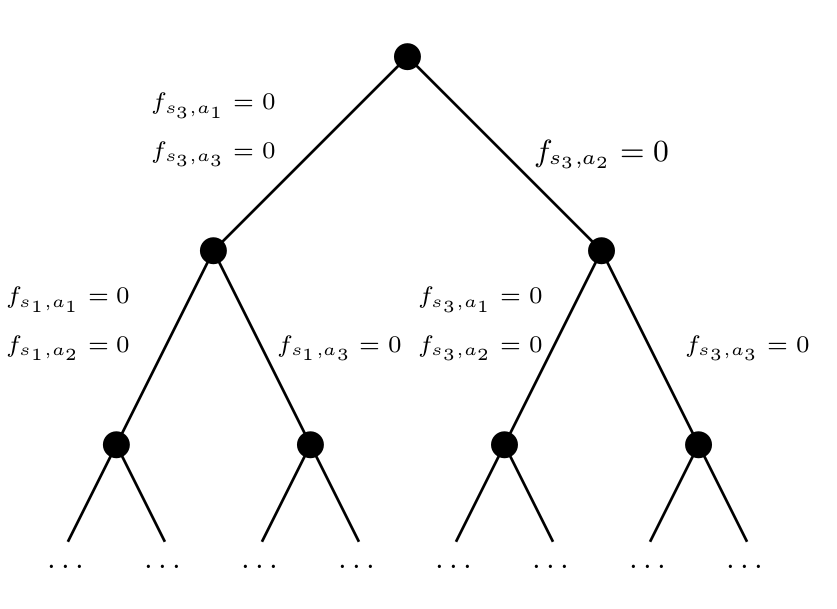
\includegraphics[scale=0.24]{images/bb.png}
	\end{center}
	\vspace{-0.5cm}
\caption{Example with  $3$ actions per state}
\end{figure}

\end{column}
\end{columns}
\end{frame}

\begin{frame}
\frametitle{\textit{Benders Decomposition} + \textit{Branch-and-Bound}}
We propose \textbf{Cut-and-branch}, an improved version of the algorithm.

\begin{itemize}
\item The \imp{root node} of the branch-and-bound tree is \imp{solved as usual}.
\item In \imp{other nodes} of the branch-and-bound tree: \imp{additional Benders cuts} are added \imp{only
if the policy found by the master problem is deterministic}. \\
%%(in this way we are sure to compute correctly the value of the maximum regret of a deterministic solution).
\pause
\item \textbf{PRO}: the time needed to process a node is lower.
\pause
\item  \textbf{CON}: the lower bound obtained is weaker (usually more nodes are explored).
\pause
\item[] $\Rightarrow$ we explore more nodes but faster.
\end{itemize}
\end{frame}



\section[Theoretical analysis]{Theoretical analysis}

\begin{frame}
\frametitle{\textit{Determinised} policy}
\begin{itemize}
\item We want to obtain a deterministic policy from a stochastic policy.
\item \textbf{Basic idea}: if only one action is possible for each state, we assume that the most probable action should be chosen. 
\end{itemize}

\begin{block}{Determinised policy}
Let $\tilde{f}$ be a given visitation frequency value for the optimal stochastic policy. The corresponding ``rounding'' determinised policy $\hat{\pi}$ can be computed as follows:
\begin{itemize}
\item for each $s'\in S$:
\begin{itemize}
\item find the action \imp{$a' = \text{argmax}_{a \in A}f_{s',a}$}.
\item fix the rest of the action to zero: $\hat{f}_{s',a} =0, \forall a \neq a'$
\end{itemize}
\item recover the deterministic policy $\hat{\pi}$ obtained from the above fixing $\hat{f}$.
\end{itemize} 
\end{block}
\end{frame}

\begin{frame}
\frametitle{\textit{Determinised} policy}

\begin{theorem}
The ratio between the maximum regret of the determinised policy and the optimal deterministic policy can be at least equal to $2$
\end{theorem}

\begin{itemize}
\item The theorem confirms that using this “common sense” idea of adapting
a stochastic policy can lead to \imp{solution significantly sub-optimal}.
\end{itemize}	
\end{frame}

\section[Experimental results]{Experimental results}

\begin{frame}
\frametitle{Instance description}
\begin{itemize}
\item Random MDPs, unlimited connections (\texttt{Random-unlim}).\\
 From the literature.
\item Random MDPs, limited connections (\texttt{Random-lim}).\\
 New set of instances.
\item Diamond MDPs (\texttt{Diamond}).\\
 From the literature and new.
\end{itemize}
\begin{block}{Value Ratio ($VR$)}
Let $MR(f^{\hat{\pi}}, \mathcal{R})$ be the maximum regret of the determinised policy and $MR(f^{\pi^*}, \mathcal{R})$  be the maximum regret of the optimal deterministic policy.\\

We define the \textit{Value Ratio} of such MDPs as: $VR = \dfrac{MR(f^{\hat{\pi}}, \mathcal{R})}{MR(f^{\pi^*}, \mathcal{R})}\;$.
\end{block}
\end{frame}


\begin{frame}
\frametitle{Experimental results - VR}
\begin{overlayarea}{\textwidth}{6cm}
    \only<1>{
    
\begin{table}[h]																					
\centering																					
\small																					
\setlength{\tabcolsep}{4.0pt}																					
\renewcommand	\arraystretch{1.1}																				
\begin{tabular}{cccccccccccccccccc}																					
\texttt{|S|}	&	5	&	 	&	 	&	 	&	 	&	10	&	 	&	 	&	 	&	 	\\
%%\cmidrule(lr){1-1} \cmidrule(lr){2-6} \cmidrule(lr){7-11}																					
\texttt{|A|}	&	2	&	3	&	4	&	5	&	10	&	2	&	3	&	4	&	5	&	10	\\
\cmidrule(lr){1-1} \cmidrule(lr){2-6} \cmidrule(lr){7-11}																					
\texttt{VR}, Avg. &		1.07	&	1.03	&	1.09	&	1.07	&	1.02	&	1.11	&	1.15	&	1.04	&	1.06	&	1.01	\\
\texttt{VR}, Max. &		1.58	&	1.28	&	1.44	&	1.34	&	1.08	&	1.27	&	1.78	&	1.13	&	1.18	&	1.03	
\end{tabular}																					
\caption{Value Ratio for \texttt{Random-unlim} MDPs.}
\label{tab random}
\end{table}																					
  
\begin{table}[h]																									
\centering																									
\scriptsize																									
\setlength{\tabcolsep}{2.5pt}																									
\renewcommand	\arraystretch{1.1}																								
\begin{tabular}{cccccccccccccccccccccc}																									
\texttt{|S|}	&	5	&	 	&	6	&	 	&	7	&		&	8	&	 	&	9	&	 	&	10	&		\\
%%\cmidrule(lr){1-1} \cmidrule(lr){2-6} \cmidrule(lr){7-11}																									
\texttt{|A|}	&	3	&	6	&	3	&	6	&	3	&	6	&	3	&	6	&	3	&	6	&	3	&	6	\\
\cmidrule(lr){1-1} \cmidrule(lr){2-3} \cmidrule(lr){4-5} \cmidrule(lr){6-7} \cmidrule(lr){8-9} \cmidrule(lr){10-11} \cmidrule(lr){12-13}
\texttt{VR}, Avg. &		1.10	&	1.11	&	1.23	&	1.09	&	1.11	&	1.55	&	1.42	&	1.20	&	1.17	&	1.11	&	1.07	&	1.14	\\
\texttt{VR}, Max. &		1.29	&	1.35	&	1.68	&	1.14	&	1.45	&	2.76	&	1.87	&	1.96	&	1.74	&	1.29	&	1.21	&	1.33	
\end{tabular}																									
\caption{Value Ratio for \texttt{Random-lim} MDPs.}																									
\label{tab:random_trident_slim}																									
\end{table}																									
  
    }
        \only<2>{
\begin{table}[h]																	
 \centering
 \small
 \setlength{\tabcolsep}{4.0pt}
 \renewcommand \arraystretch{1.1}
\begin{tabular}{ccccccccccc}																					
\texttt{p}	&	5	&	10	&	15	&	20	&	25	&	30	&	35	&	40	&	45	 \\	
\cmidrule(lr){1-1} \cmidrule(lr){2-10} \cmidrule(lr){11-11}
\texttt{VR} &	1.66	&	1.24	&	1.16	&	1.13	&	1.15	&	1.15	&	1.15	&	1.14	&	1.16 
\end{tabular}
\caption{Value Ratio for \texttt{Diamond}.}
\label{tab:diamond_slim}								
\end{table}																						
  
    }
\end{overlayarea}
\end{frame}


\begin{frame}
\frametitle{Experimental results - cut-and-branch}


\begin{overlayarea}{\textwidth}{6cm}
    \only<1>{
%%%%%%%%%%%%%%%%%
\begin{figure}[]
	\begin{center}
    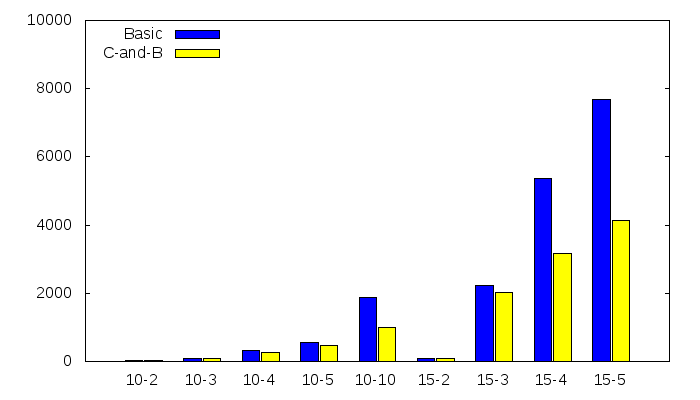
\includegraphics[scale=0.45]{GNUPLOT/output_random.png}
	\end{center}
	\caption{Impact of cut-and-branch, \texttt{Random-unlim} MDPs (states-actions vs computing time, in seconds).}
	\label{fig:impact_random} 
\end{figure}
%%%%%%%%%%%%%%%%%
    }
        \only<2>{
%%%%%%%%%%%%%%%%%
\begin{figure}[]
	\begin{center}
    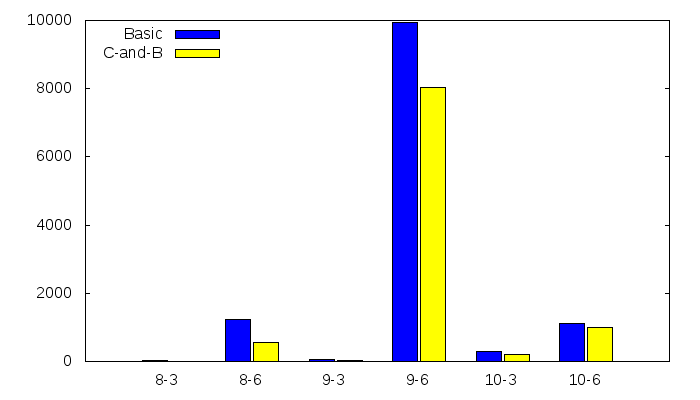
\includegraphics[scale=0.45]{GNUPLOT/output_trident.png}
	\end{center}
	\caption{Impact of cut-and-branch, \texttt{Random-lim} MDPs (states-actions vs computing time, in seconds).}
	\label{fig:impact_trident} 
\end{figure}
%%%%%%%%%%%%%%%%%
    }
\end{overlayarea}



\end{frame}



\section[Conclusions]{Conclusions}

\begin{frame}
\frametitle{Conclusions}
\end{frame}
\end{document}
